\documentclass[margin=5mm]{standalone}
\usepackage[utf8]{inputenc}
\usepackage{tikz}
\usetikzlibrary{matrix,positioning}

\tikzset{
  tab/.style={inner sep=0pt,
    nodes={inner sep=.333em,
      % notwendig für leere Zellen und Unterlängen:
      minimum height={\baselineskip+0.666em}
    }
  },
  vtab/.style={matrix of nodes,tab,
    row sep=-\pgflinewidth,column sep=-\pgflinewidth,
    nodes in empty cells,% leere Zellen werden ebenfalls gezeichnet
    nodes={draw,align=left,text width=#1}
  },
  vtab/.default=3cm,% voreingestellte Breite
  htab/.style={matrix of nodes,draw,tab,anchor=north west},
  every edge/.append style={font=\footnotesize\strut,inner ysep=.1em},
  pfeil/.style={out=270,in=90,->}
}

\begin{document}
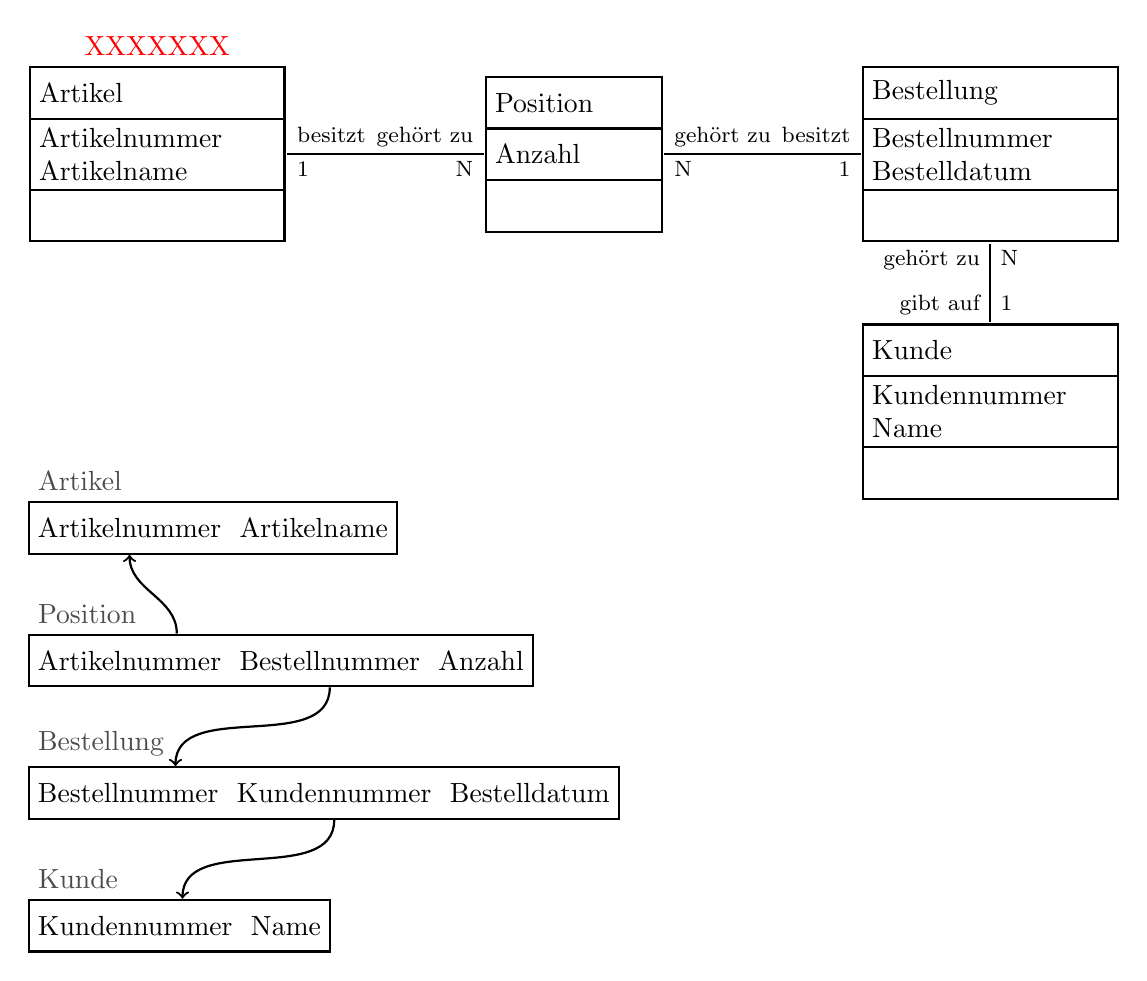
\begin{tikzpicture}[thick,
  % vertikaler und horizontaler Abstand zwischen den Tabellen:
  node distance=1cm and 2.5cm, 
]
% Tabellen
  \matrix(A)[vtab] {Artikel\\{Artikelnummer\newline Artikelname}\\\\};
\node [red,above] at (A-1-1.north) {XXXXXXX};
  % für matrix P reichen 2cm als Breite
  \matrix(P)[right= of A,vtab=2cm]{Position\\Anzahl\\\\};
  \matrix(B)[right= of P,vtab]{Bestellung\\{Bestellnummer\newline Bestelldatum}\\\\};
  \matrix(K)[below= of B,vtab]{Kunde\\{Kundennummer\newline Name}\\\\};
% Verbindungen einzeichnen und beschriften
    \path(A)edge
      node[pos=0,above right]{besitzt}node[pos=0,below right]{1}
      node[pos=1,above left]{gehört zu}node[pos=1,below left]{N}
      (P);
    \path(P)edge
      node[pos=0,above right]{gehört zu}node[pos=0,below right]{N}
      node[pos=1,above left]{besitzt}node[pos=1,below left]{1}
      (B);
    \path(B)edge
      node[pos=0,below left]{gehört zu}node[pos=0,below right]{N}
      node[pos=1,above left]{gibt auf}node[pos=1,above right]{1}
      (K);
%
% horizontale Tabellen
  \matrix(a)[htab]at(A.west|-K.south){Artikelnummer&Artikelname\\};
  \matrix(p)[below=of a.south west,htab]{Artikelnummer&Bestellnummer& Anzahl\\};
  \matrix(b)[below=of p.south west,htab]{ Bestellnummer&Kundennummer&Bestelldatum\\};
  \matrix(k)[below=of b.south west,htab]{Kundennummer& Name\\};
% Beschriftung der Tabellen
  \foreach \t/\bez in {a/Artikel,p/Position,b/Bestellung,k/Kunde}
    \node[above right=0pt of \t.north west,text=black!70]{\bez};
% Verbindungen einzeichnen
  % Pfeile enden um xshift in x-Richtung verschoben am Nordanker des Zielknotens.
  % Verschiebung ist notwendig, damit die Pfeile nicht über der Beschriftung liegen.
  \path[pfeil,<-](a-1-1)edge([xshift=.6cm]p-1-1.north);
  \path[pfeil](p-1-2)edge([xshift=.6cm]b-1-1.north);
  \path[pfeil](b-1-2)edge([xshift=.6cm]k-1-1.north);
\end{tikzpicture}
\end{document}